\tikzset{every picture/.style={line width=0.75pt}} %set default line width to 0.75pt        

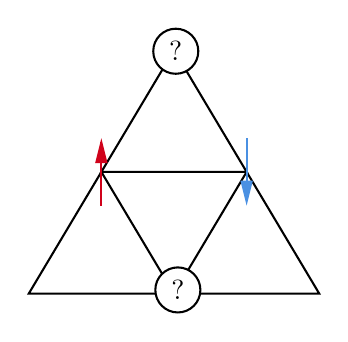
\begin{tikzpicture}[x=0.75pt,y=0.75pt,yscale=-1,xscale=1]
%uncomment if require: \path (0,300); %set diagram left start at 0, and has height of 300

%Shape: Triangle [id:dp3265971145624944] 
\draw   (225,126.33) -- (260,185) -- (190,185) -- cycle ;
%Shape: Triangle [id:dp457754747303309] 
\draw   (155,126.33) -- (190,185) -- (120,185) -- cycle ;
%Shape: Triangle [id:dp5282716496110524] 
\draw   (190,67.66) -- (225,126.33) -- (155,126.33) -- cycle ;
%Straight Lines [id:da7008008238341734] 
\draw [color={rgb, 255:red, 208; green, 2; blue, 27 }  ,draw opacity=1 ]   (155,142.56) -- (155,112.1) ;
\draw [shift={(155,110.1)}, rotate = 450] [fill={rgb, 255:red, 208; green, 2; blue, 27 }  ,fill opacity=1 ][line width=0.08]  [draw opacity=0] (12,-3) -- (0,0) -- (12,3) -- cycle    ;
%Straight Lines [id:da47122065737438956] 
\draw [color={rgb, 255:red, 74; green, 144; blue, 226 }  ,draw opacity=1 ]   (225,110.1) -- (225,140.56) ;
\draw [shift={(225,142.56)}, rotate = 270] [fill={rgb, 255:red, 74; green, 144; blue, 226 }  ,fill opacity=1 ][line width=0.08]  [draw opacity=0] (12,-3) -- (0,0) -- (12,3) -- cycle    ;
%Shape: Circle [id:dp2858034795038058] 
\draw  [fill={rgb, 255:red, 255; green, 255; blue, 255 }  ,fill opacity=1 ] (181,183.18) .. controls (181,177.19) and (185.86,172.33) .. (191.85,172.33) .. controls (197.85,172.33) and (202.71,177.19) .. (202.71,183.18) .. controls (202.71,189.18) and (197.85,194.04) .. (191.85,194.04) .. controls (185.86,194.04) and (181,189.18) .. (181,183.18) -- cycle ;

%Shape: Circle [id:dp48141040110301847] 
\draw  [fill={rgb, 255:red, 255; green, 255; blue, 255 }  ,fill opacity=1 ] (180,68.18) .. controls (180,62.19) and (184.86,57.33) .. (190.85,57.33) .. controls (196.85,57.33) and (201.71,62.19) .. (201.71,68.18) .. controls (201.71,74.18) and (196.85,79.04) .. (190.85,79.04) .. controls (184.86,79.04) and (180,74.18) .. (180,68.18) -- cycle ;


% Text Node
\draw (191.85,183.18) node   [align=left] {?};
% Text Node
\draw (190.85,68.18) node   [align=left] {?};


\end{tikzpicture}